%%%%%%%%%%%%%%%%%%%%%%%%%%%%%%%%%%%%%%%%%%%%%%%%%
\section{Faire des animations}
\begin{frame} [fragile]
  \frametitle{Exemple avec tikZ - v1}
\begin{center}
  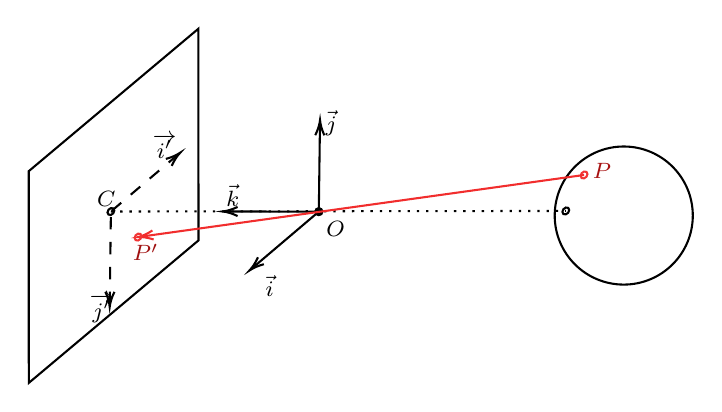
\begin{tikzpicture}[x=0.50pt,y=0.50pt,yscale=-1,xscale=1]
  %uncomment if require: \path (0,300); %set diagram left start at 0, and has height of 300
    \visible<1->{
      %Shape: Circle [id:dp2644497771544846] 
      \draw  [color={rgb, 255:red, 241; green, 53; blue, 53 }  ,draw opacity=1 ] (512.82,105.92) .. controls (514.18,105.55) and (515.28,106.36) .. (515.28,107.72) .. controls (515.28,109.09) and (514.18,110.49) .. (512.82,110.85) .. controls (511.45,111.22) and (510.35,110.41) .. (510.35,109.05) .. controls (510.35,107.68) and (511.45,106.28) .. (512.82,105.92) -- cycle ;
      %Shape: Circle [id:dp3002036179403492] 
      \draw   (491.6,137.7) .. controls (491.6,110.14) and (513.94,87.8) .. (541.5,87.8) .. controls (569.06,87.8) and (591.4,110.14) .. (591.4,137.7) .. controls (591.4,165.26) and (569.06,187.6) .. (541.5,187.6) .. controls (513.94,187.6) and (491.6,165.26) .. (491.6,137.7) -- cycle ;

      % Text Node
      \draw (517,97.9) node [anchor=north west][inner sep=0.75pt]  [font=\footnotesize,color={rgb, 255:red, 167; green, 17; blue, 17 }  ,opacity=1 ]  {$P$};


      \tikzset{every picture/.style={line width=0.75pt}} %set default line width to 0.75pt        
    }
    \visible<2->{

      %Shape: Circle [id:dp1706683186516259] 
      \draw  [fill={rgb, 255:red, 0; green, 0; blue, 0 }  ,fill opacity=1 ] (321.12,132.42) .. controls (322.48,132.42) and (323.58,133.52) .. (323.58,134.88) .. controls (323.58,136.25) and (322.48,137.35) .. (321.12,137.35) .. controls (319.75,137.35) and (318.65,136.25) .. (318.65,134.88) .. controls (318.65,133.52) and (319.75,132.42) .. (321.12,132.42) -- cycle ;
      %Straight Lines [id:da37723246736535] 
      \draw    (321.12,134.88) -- (321.97,70.75) ;
      \draw [shift={(322,68.75)}, rotate = 90.77] [color={rgb, 255:red, 0; green, 0; blue, 0 }  ][line width=0.75]    (10.93,-3.29) .. controls (6.95,-1.4) and (3.31,-0.3) .. (0,0) .. controls (3.31,0.3) and (6.95,1.4) .. (10.93,3.29)   ;
      %Straight Lines [id:da8292136284936239] 
      \draw    (321.12,134.88) -- (253.5,134.75) ;
      \draw [shift={(251.5,134.75)}, rotate = 0.11] [color={rgb, 255:red, 0; green, 0; blue, 0 }  ][line width=0.75]    (10.93,-3.29) .. controls (6.95,-1.4) and (3.31,-0.3) .. (0,0) .. controls (3.31,0.3) and (6.95,1.4) .. (10.93,3.29)   ;
      %Straight Lines [id:da997223962826064] 
      \draw    (321.12,134.88) -- (272.48,176.16) ;
      \draw [shift={(270.95,177.45)}, rotate = 319.68] [color={rgb, 255:red, 0; green, 0; blue, 0 }  ][line width=0.75]    (10.93,-3.29) .. controls (6.95,-1.4) and (3.31,-0.3) .. (0,0) .. controls (3.31,0.3) and (6.95,1.4) .. (10.93,3.29)   ;

      % Text Node
      \draw (324,59.9) node [anchor=north west][inner sep=0.75pt]  [font=\footnotesize]  {$\vec{j}$};
      % Text Node
      \draw (280.5,178.9) node [anchor=north west][inner sep=0.75pt]  [font=\footnotesize]  {$\vec{i}$};
      % Text Node
      \draw (324.43,139.84) node [anchor=north west][inner sep=0.75pt]  [font=\footnotesize]  {$O$};
      % Text Node
      \draw (252,112.9) node [anchor=north west][inner sep=0.75pt]  [font=\footnotesize]  {$\vec{k}$};
    }

    \visible<3->{

      \tikzset{every picture/.style={line width=0.75pt}} %set default line width to 0.75pt        


      %Shape: Rectangle [id:dp2954760785671301] 
      \draw  [line width=0.75]  (234.11,2.68) -- (234.16,155.68) -- (111.53,258.66) -- (111.47,105.66) -- cycle ;
      %Shape: Circle [id:dp8031961960387121] 
      \draw   (170.87,132.32) .. controls (172.23,131.96) and (173.33,132.77) .. (173.33,134.13) .. controls (173.33,135.49) and (172.23,136.89) .. (170.87,137.26) .. controls (169.5,137.62) and (168.4,136.81) .. (168.4,135.45) .. controls (168.4,134.09) and (169.5,132.69) .. (170.87,132.32) -- cycle ;
      %Straight Lines [id:da5095252202259546] 
      \draw  [dash pattern={on 0.84pt off 2.51pt}]  (170.87,134.79) -- (499.62,134.38) ;
      %Shape: Circle [id:dp6766149755736347] 
      \draw   (499.62,131.92) .. controls (500.98,131.55) and (502.08,132.36) .. (502.08,133.72) .. controls (502.08,135.09) and (500.98,136.49) .. (499.62,136.85) .. controls (498.25,137.22) and (497.15,136.41) .. (497.15,135.05) .. controls (497.15,133.68) and (498.25,132.28) .. (499.62,131.92) -- cycle ;
      %Straight Lines [id:da02893381123300387] 
      \draw  [dash pattern={on 4.5pt off 4.5pt}]  (170.03,201.75) -- (170.87,134.79) ;
      \draw [shift={(170,203.75)}, rotate = 270.72] [color={rgb, 255:red, 0; green, 0; blue, 0 }  ][line width=0.75]    (10.93,-3.29) .. controls (6.95,-1.4) and (3.31,-0.3) .. (0,0) .. controls (3.31,0.3) and (6.95,1.4) .. (10.93,3.29)   ;
      %Straight Lines [id:da9780084753446128] 
      \draw  [dash pattern={on 4.5pt off 4.5pt}]  (219.51,93.52) -- (170.87,134.79) ;
      \draw [shift={(221.03,92.22)}, rotate = 139.68] [color={rgb, 255:red, 0; green, 0; blue, 0 }  ][line width=0.75]    (10.93,-3.29) .. controls (6.95,-1.4) and (3.31,-0.3) .. (0,0) .. controls (3.31,0.3) and (6.95,1.4) .. (10.93,3.29)   ;

      % Text Node
      \draw (158.65,118.28) node [anchor=north west][inner sep=0.75pt]  [font=\footnotesize]  {$C$};
      % Text Node
      \draw (199,76.9) node [anchor=north west][inner sep=0.75pt]  [font=\footnotesize]  {$\overrightarrow{i'}$};
      % Text Node
      \draw (153.5,192.4) node [anchor=north west][inner sep=0.75pt]  [font=\footnotesize]  {$\overrightarrow{j'}$};
    }

    \visible<4->{
      \tikzset{every picture/.style={line width=0.75pt}} %set default line width to 0.75pt        

      %Shape: Circle [id:dp1451724167499565] 
      \draw  [fill={rgb, 255:red, 0; green, 0; blue, 0 }  ,fill opacity=1 ] (321.12,132.42) .. controls (322.48,132.42) and (323.58,133.52) .. (323.58,134.88) .. controls (323.58,136.25) and (322.48,137.35) .. (321.12,137.35) .. controls (319.75,137.35) and (318.65,136.25) .. (318.65,134.88) .. controls (318.65,133.52) and (319.75,132.42) .. (321.12,132.42) -- cycle ;
      %Straight Lines [id:da16865708500122678] 
      \draw [color={rgb, 255:red, 241; green, 45; blue, 45 }  ,draw opacity=1 ]   (512.82,108.38) -- (192.48,152.97) ;
      \draw [shift={(190.5,153.25)}, rotate = 352.08] [color={rgb, 255:red, 241; green, 45; blue, 45 }  ,draw opacity=1 ][line width=0.75]    (10.93,-3.29) .. controls (6.95,-1.4) and (3.31,-0.3) .. (0,0) .. controls (3.31,0.3) and (6.95,1.4) .. (10.93,3.29)   ;
      %Shape: Circle [id:dp8576525819791565] 
      \draw  [color={rgb, 255:red, 241; green, 53; blue, 53 }  ,draw opacity=1 ] (190.5,150.78) .. controls (191.86,150.42) and (192.97,151.23) .. (192.97,152.59) .. controls (192.97,153.95) and (191.86,155.35) .. (190.5,155.72) .. controls (189.14,156.08) and (188.03,155.27) .. (188.03,153.91) .. controls (188.03,152.55) and (189.14,151.15) .. (190.5,150.78) -- cycle ;

      % Text Node
      \draw (184.5,155.9) node [anchor=north west][inner sep=0.75pt]  [font=\footnotesize,color={rgb, 255:red, 159; green, 16; blue, 16 }  ,opacity=1 ]  {$P'$};
    }
  \end{tikzpicture}

\end{center}
\begin{flushleft}
  \visible<1->{
    $P$ : point réel\\
  }
  \visible<2->{
    $O$ : objectif de la caméra.\\
    $(i,j,k)$ : axes du repères associées à la caméra.\\
  }
  \visible<3->{
    $\pi$ : plan image de la caméra\\
  }
  \visible<4->{
    $P'$ : point image de P\\
  }
\end{flushleft}

\end{frame}